\section{Mengenlehre}

\subsection{Definition Menge}

Eine Menge ist eine wohl bestimmte Zusammenfassung von Objekten. Die
Objekte heißen \emph{Elemente} der Menge.

\begin{description}[style=nextline]
	\item[\(x \in A\)] \(x\) ist Element der Menge \(A\)
	\item[\(x \notin A\)]  \(x\) ist nicht Element der Menge \(A\)
\end{description}

\subsection{Darstellungen}

\begin{description}[style=nextline]
	\item[Aufzählung]
	\( A = \{a, e, i, o, u\} \)
	\item[Beschreibung]
	\( M = \{ x \mid x \text{ hat die Eigenschaft } E\} \)
	\item[Mengendiagramm]
	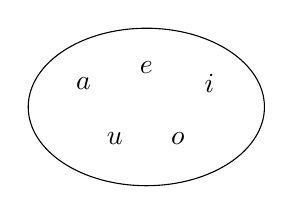
\begin{tikzpicture}
		\draw[] (0,0) ellipse (1.5cm and 1cm);
		\node[] at (-0.8, 0.3) {\(a\)};
		\node[] at (0, 0.5) {\(e\)};
		\node[] at (0.8, 0.3) {\(i\)};
		\node[] at (0.4, -0.4) {\(o\)};
		\node[] at (-0.4, -0.4) {\(u\)};
	\end{tikzpicture}
\end{description}

\subsection{Beziehungen}

\begin{description}[style=nextline]
	\item[\(A = B\)]
	\(A\) und \(B\) sind gleich, wenn sie dieselben Elemente enthalten.
	\item[\(A \subset B\)]
	\(A\) ist echte Teilmenge von \(B\), wenn jedes Element von \(A\) auch
	in \(B\) ist und \(A\) verschieden von \(B\) ist.
\end{description}


\subsection{Operationen}

\begin{description}[style=nextline]
	\item[\(A \cap B\)]
	\textbf{Schnittmenge} von \(A\) und \(B\)
	\item[\(A \cup B\)]
	\textbf{Vereinigung} von \(A\) und \(B\)
	\item[\(A \setminus B\)]
	\textbf{Differenz}, \(A\) ohne \(B\)
	\item[\(\bar{A}\)]
	\textbf{Komplement} von \(A\)
\end{description}
